%%%%%%%%%%%%%%%%%%%%%%%%%%%%%%%%%%%%%%%%%%%%%%%%%%%%%%%%%%%%%%%%%%%%%%%%%%%%%%%%
%2345678901234567890123456789012345678901234567890123456789012345678901234567890
%        1         2         3         4         5         6         7         8

%\documentclass[letterpaper, 10 pt, conference]{ieeeconf}  % Comment this line out
                                                          % if you need a4paper
\documentclass[a4paper, 10pt, conference]{ieeeconf}      % Use this line for a4
                                                          % paper

\IEEEoverridecommandlockouts                              % This command is only
                                                          % needed if you want to
                                                          % use the \thanks command
\overrideIEEEmargins
% See the \addtolength command later in the file to balance the column lengths
% on the last page of the document

% This is needed to prevent the style file preventing citations from linking to 
% the bibliography
\makeatletter
\let\NAT@parse\undefined
\makeatother

\usepackage[dvipsnames]{xcolor}

\newcommand*\linkcolours{ForestGreen}

\usepackage{times}
\usepackage{graphicx}
\usepackage{amssymb}
\usepackage{gensymb}
\usepackage{amsmath}
\usepackage{breakurl}
\def\UrlBreaks{\do\/\do-}
\usepackage{url,hyperref}
\hypersetup{
colorlinks,
linkcolor=\linkcolours,
citecolor=\linkcolours,
filecolor=\linkcolours,
urlcolor=\linkcolours}

\usepackage{algorithm}
\usepackage{algorithmic}

\usepackage[labelfont={bf},font=small]{caption}
\usepackage[none]{hyphenat}

\usepackage{mathtools, cuted}

\usepackage[noadjust, nobreak]{cite}
\def\citepunct{,\,} % Style file defaults to listing references separately

\usepackage{tabularx}
\usepackage{amsmath}

\usepackage{float}

\usepackage{pifont}% http://ctan.org/pkg/pifont
\newcommand{\cmark}{\ding{51}}%
\newcommand{\xmark}{\ding{55}}%

\newcommand*\diff{\mathop{}\!\mathrm{d}}
\newcommand*\Diff[1]{\mathop{}\!\mathrm{d^#1}}
\newcommand*\imgres{600}

\newcommand*\GitHubLoc{https://github.com/Jeffrey-Ede/ALRC}

\newcolumntype{Y}{>{\centering\arraybackslash}X}

%\usepackage{parskip}

\usepackage[]{placeins}

% \usepackage{epstopdf}
% \epstopdfDeclareGraphicsRule{.tif}{png}{.png}{convert #1 \OutputFile}
% \AppendGraphicsExtensions{.tif}

\newcommand\extraspace{3pt}

\usepackage{placeins}

\usepackage{tikz}
\newcommand*\circled[1]{\tikz[baseline=(char.base)]{
            \node[shape=circle,draw,inner sep=0.8pt] (char) {#1};}}
            
\usepackage[framemethod=tikz]{mdframed}

\usepackage{afterpage}

\usepackage{stfloats}

\usepackage{atbegshi}
\newcommand{\handlethispage}{}
\newcommand{\discardpagesfromhere}{\let\handlethispage\AtBeginShipoutDiscard}
\newcommand{\keeppagesfromhere}{\let\handlethispage\relax}
\AtBeginShipout{\handlethispage}

\usepackage{comment}

\title{\LARGE \bf
Time-series Analysis on Cryptocurrency Pricing and its relationship with Economic Factors in a post-COVID world.
}

\author{ \parbox{3 in}{\centering Chin Phin Ong\\
          School of Physics and Astronomy\\
          University of Southampton}}

\begin{document}

\maketitle
\thispagestyle{empty}
\pagestyle{empty}

%%%%%%%%%%%%%%%%%%%%%%%%%%%%%%%%%%%%%%%%%%%%%%%%%%%%%%%%%%%%%%%%%%%%%%%%%%%%%%%%
\begin{abstract}

This project delves into the dynamics of cryptocurrency markets, particularly focusing on Bitcoin (BTC) and its relationships with other cryptocurrencies, as well as external factors such as search popularity and traditional financial indices after the pandemic (2021-2023). Using time-series analysis techniques, I explore the correlations and time-lags between BTC and selected cryptocurrencies (ETH, SOL, LTC, USDT), as well as BTC's relationship with Google search trends, the S\&P500 index, gold prices, and the EUR-USD exchange rate. Positive monotonic relationships between BTC and most cryptocurrencies were observed, with negligible time lags on the scale of days. Additionally, I observe a positive correlation between BTC prices and search popularity, as well as with the S\&P500 index, indicating potential influences from broader economic trends. However, no significant relationships were found between BTC and gold prices or the EUR-USD exchange rate.

\end{abstract}

%%%%%%%%%%%%%%%%%%%%%%%%%%%%%%%%%%%%%%%%%%%%%%%%%%%%%%%%%%%%%%%%%%%%%%%%%%%%%%%%
\section{Introduction}
As cryptocurrency continues to grow in popularity, especially during the COVID-19 pandemic, where people have realised the importance of investing and have looked into cryptocurrency as a viable investment \cite{Corbet2018}. In this project, I will explore the correlation between the values between 2021-2023 of some of the top cryptocurrencies - BTC (Bitcoin), ETH (Ethereum), USDT (Tether USD), and SOL (Solana) based on their market caps\footnote{Based on: \url{https://coinmarketcap.com/}, May 2024.} (the total market value of a cryptocurrency's circulating supply.). BTC is the most popular cryptocurrency on the market, with a market cap of 1.2 trillion USD (May 2024). It was introduced in \cite{Nakamoto2008} as a way to send digital payments via peer-to-peer (P2P) method without passing through a middle-man (e.g., a bank or broker) to prevent "double-spending" - having to pay additional costs on top of the transaction\footnote{According to \cite{Nakamoto2008}, "financial institutions cannot avoid mediating disputes", therefore the cost of the mediation brings up the transaction costs.}. Since then, many other cryptocurrencies have entered the market. As of April 2024, there are over \textbf{2.4 million} cryptocurrencies on the market, with an average of 5,300 launched daily\footnote{Source: \url{https://www.coingecko.com/research/publications/how-many-cryptocurrencies-are-there}.}.

Among them, some notable cryptocurrencies are ETH, USDT, LTC and DOGE. Each of these coins (a term used interchangeably with cryptocurrency) have their unique properties. Ethereum uses a proof-of-stake consensus model\footnote{\url{https://ethereum.org/en/developers/docs/consensus-mechanisms/}}, which is different from the proof-of-work model used by Bitcoin. USDT is a "stablecoin" that is pegged to the value of the US dollar, making it less volatile than other cryptocurrencies. These properties and features of each cryptocurrency can impact their use cases and potential for adoption in various industries.

Numerous studies have investigated the properties of such cryptocurrencies - the seasonality\footnote{The tendency for the cryptocurrency/asset to perform better in certain times compared to others - this can be on the time scale of days, weeks, months, half-years or years. Source: \url{https://corporatefinanceinstitute.com/resources/valuation/seasonality/}. Apart from finance, there have been studies in psychology analysing the seasonality of schizophrenia patient admissions \cite{Yao2023}.} \cite{Kaiser2019}, hedging ability \cite{Chan2019}, multifractality\footnote{The property of complex systems where irregular patterns or structures exhibit varying degrees of complexity across different scales, extending the concept of fractals to multiple scales of organization - e.g. seeing a pattern that changes in how detailed or messy it looks depending on how closely you're looking at it. For more information, read to \cite{Harte2001}} \cite{Takaishi2018}, interdependence between \cite{Qureshi2020} and even the environmental impact \cite{Wendl2023, Mohsin2021, Corbet2020} of cryptocurrencies. On the other hand, \cite{Georgoula2015} studied how Twitter, Wikipedia search queries, hash rates, USD/EUR\footnote{United States Dollar to Euro} exchange rate, number of coins in circulation, S\&P500 index (state of the global economy) affected the price of Bitcoin.

One way that financial data can be analysed is via time-series analysis. This method has been used to analyse the stock market - \cite{cao1992nonlinear, naik2013does, parray2020time}, as well as cryptocurrencies - \cite{Georgoula2015, Catania2017, Hagemann2018, Maleki2023, Vaz2020, Toyoda2018}. With an appropriate time scale, some observations between cryptocurrency pairs, crypto-stock pairings, crypto-query (search query) pairings can be done.\footnote{\cite{Pal2017} is a good resource on basic practical time-series methods.}

In this project, the questions that I will explore and answer in the following sections are:
\begin{enumerate}
    \item Is there any correlation between the time series of cryptocurrency pairings? To what degree are they correlated? %correlation
    \item Is there any observable lag between them? %correlation
    \item What about the stock market? What is the correlation between these cryptocurrencies, i.e. BTC against the S\&P 500 (SPX), or BTC against gold spot\footnote{Gold spot prices are typically quoted as USD per troy ounce, about $0.03kg$} prices (XAU)?
    \item Does the popularity (based on Google search trends) of BTC influence the price of BTC, or is it the other way round?
\end{enumerate}

In the following sections, I will describe the methodology used to answer the questions. Then, I will present the results that answer the questions above and thoroughly analyse them. Finally, I will offer a brief conclusion on the findings of this project and discuss future work.

\section{Methodology}
One of the main tools used in time-series analysis is correlation. Correlation is the relationship between two sets of data. In this project, I will be using the Spearman correlation coefficient  Methods are taken from \cite{Pal2017}
\subsection{Processing Data}
The time scales of the data are from the beginning of 2021 to 2023. The historical price data of the cryptocurrencies are downloaded from \url{https://www.cryptodatadownload.com/data/bitstamp/}, and historical stock prices are downloaded from \url{nasdaq.com}, where the daily closing prices of the assets are taken. Search popularity data is taken from \url{https://trends.google.co.uk/trends/explore?date=today\%205-y&q=\%2Fm\%2F05p0rrx&hl=en}. EUR-USD exchange rate data is from \url{www.macrotrends.net}.

\subsection{Pearson Correlation Coefficient}\label{Pearson}
The Pearson correlation coefficient measures the monotonic\footnote{"monotonic" carries a similar relationship to the word "linear", but it is not the same. It means that the behaviour of data moves in a direction that is constantly increasing/decreasing but does not follow the linear equation $y = mx + b$.} relationship between two variables, ranging from $-1$ to $1$. $-1$ indicates perfect negative linear relationship, $1$ indicates perfect linear relationship, and $0$ represents no  linear relationship \cite{Dowdy1983}. The correlation coefficient, $\rho_{p}$, for two vectors $x$ and $y$ is:
\begin{equation}
    \rho_{p} = \frac{\sum(x-m_x)(y-m_y)}{\sqrt{\sum(x-m_x)^2\sum(y-m_y)^2}}
\end{equation}
Where $m_x$ and $m_y$ are means of the vectors $x$ and $y$. A positive correlation means that if $x$ increases, $y$ increases, and vice versa.

\subsection{Spearman's (Rank) Correlation Coefficient}
Similar in purpose to the Pearson Correlation Coefficient (Section \ref{Pearson}), the difference in the Spearman coefficient is that it measures the \textbf{monotonic} relationship between 2 sets of data instead of the linear relationship. By converting the raw data of the two samples, $X_i$ and $Y_i$ into ranks\footnote{"ranking" data here means arranging the data points from smallest to largest, and then ranking the datapoints relative to the rest, where the rank of 1 corresponds to the smallest data point. If two values are the same, the rank of the numbers are the average rank of where they would fall if they were different.} $R(X_i)$ and $R_(Y_i)$, the Spearman coefficient, $\rho_s$ can be obtained with:
\begin{equation}
    \rho_s = \rho_{p(R(X), R(Y))} = \frac{cov(R(X), R(Y)}{\sigma_{R(X)}\sigma_{R(Y)}}
\end{equation}

where $\rho$ is the Pearson coefficient applied to the rank variables, $cov(R(X), R(Y))$ is the covariance of the rank variables, and $\sigma_{R(X)}$ and $\sigma_{R(Y)}$ are the standard deviations of the rank variables. Between two datasets X and Y, a positive value of the Spearman correlation coefficient means that there is an increasing monotonic relationship (with 1 being perfectly increasing monotonic relationship), and a negative value indicates a decreasing monotonic relationship (with -1 being perfectly decreasing monotonic relationship), whereas 0 means there is no monotonic relationship between the two datasets. 
 
\subsection{Cross-correlation}
Cross-correlation is a measure of similarity between two signals as a function of the relative shift of one signal to another. It measures the degree to which two signals resemble each other as one signal is shifted in time relative to another. The time series data is presented as arrays. If the correlation between 2 time series, $x$ and $y$ (with length $||x||$ and $||y||$ respectively) is the array $z$, with ${k}^{th}$ element $z[{k}]$, the correlation can be written as: 
\begin{equation}
    z[{k}] = (x * y)(k - N + 1) = \sum_{l=0}^{||x||-1}x_{l}y^{*}_{l-k+N-1}
\end{equation}
for $k = 0, 1,..., ||x||+||y||-2$, $N = max(||x||, ||y||)$, $y_m = 0$ if $m > ||y||$\footnote{Source: \url{https://docs.scipy.org/doc/scipy/reference/generated/scipy.signal.correlate.html}}

\subsection{Error Handling}
According to \cite{Misra2018}, the traditional method to obtain the error on cross-correlation (or the time-lag), the signal is divided into equal segments and the cross-correlation is found for each segment. The net cross-correlation is the average of the cross-correlation of the segments, and the variance is the error. However, \cite{Misra2018} also considers data size to be "small" at $\sim1000$ data points, stating that dividing the data into segments is less practical. Therefore, I decided to do a sampling (with replacement) of the datasets, where the sample size is large\footnote{In this case, it will be the same length of the original dataset.} such that a relationship between the two datasets can be drawn \cite{Kose2023} and the standard deviation can be calculated. The standard deviation on the time lag, $\sigma_\tau$ is the standard deviation of the time lags that correspond to the maximum cross-correlation value for each cross-correlation of the sample. The standard deviation on the cross-correlation at time lag $\tau$ (not to be confused with Kendall's tau - I am not using that in this report), $\sigma_{corr}(\tau)$ is the standard deviation of the cross-correlation value for each sample at time lag $\tau$. The average standard deviation of the cross-correlation is calculated by taking the average of all $\sigma_{corr}(\tau)$ at every time $\tau$. A standard error is calculated with:
\begin{equation}
    \epsilon = \frac{\sigma}{\sqrt{n}}
\end{equation}
Where $\epsilon$ is the standard error, and $n$ is the sample size.
\section{Results}
The relationship between cryptocurrencies will be investigated from the year January 1st, 2021 to December 31st, 2023, to determine if the trend of the relationships between cryptocurrency pairs or cryptocurrency stock pairs has changed, building upon the work of \cite{Sifat2019} (BTC-ETH pairs), and \cite{Georgoula2015} (BTC-SPX, BTC-XAU), and comparing analysis to \cite{Corbet2020contagion}. The pairs investigated are BTC-ETH, BTC-LTC, BTC-SOL and BTC-USDT. It is expected that BTC-ETH to show 0 time-lag, and a positive monotonic relationship - I hypothesise this will be the case for most "popular" coins. The only cryptocurrency pair that would likely show no monotonic relationship will be the BTC-USDT pair, since the value of USDT is based off the USD, so there would be not much of a fluctuation in price relative to BTC. The two main graphs that I will show are: scatter plots which show the relationship (monotonic/non-monotonic) of the pairs of data analysed, and the cross-correlation against time-lag for all the BTC-X coin pairings. The Pearson and Spearman correlation coefficients,  will be calculated and quoted.

Some interesting data to work with are the effects on BTC based on factors that are not cryptocurrency.Results are shown in Section \ref{extras}. The areas of investigation are:
\begin{itemize}
    \item The relationship between the popularity of "Bitcoin" as a search engine term and the price of BTC
    \item The relationship between BTC pricing the S\&P500 index (which is an indicator of global economy)
    \item The relationship between BTC and the price of gold
    \item The relationship between BTC and the value of the dollar, based off the USD-EUR exchange rate \cite{Georgoula2015}
\end{itemize}

\subsection{Correlation and time-lag (cross-correlation) between cryptocurrencies}
The scatter plots of the BTC-X pairings are shown in Fig. \ref{btc-eth} to Fig. \ref{btc-usdt}:
The most popular pair is the BTC-ETH pairing. This was expected to have a monotonic relationship.
\begin{figure}
    \centering
    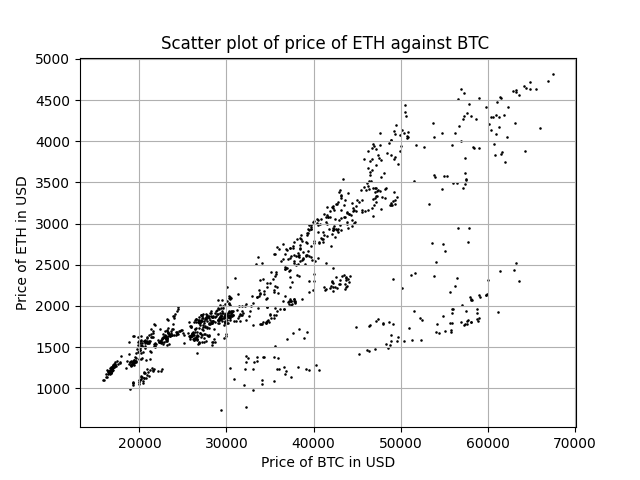
\includegraphics[width = \columnwidth]{Projects/TimeSeriesAnalysis/WrittenReport/plots/btcEth.png}
    \caption{Scatter Plot of BTC and ETH prices, Jan '21 to Dec '23.\\
    \begin{centering}
        $\rho_p = 0.786$\\
        $\rho_s = 0.819$\\
    \end{centering}}
    \label{btc-eth}
\end{figure}

\begin{figure}
    \centering
    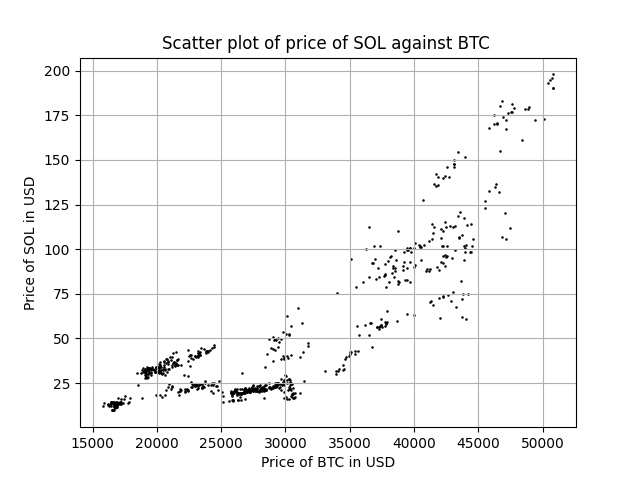
\includegraphics[width = \columnwidth]{Projects/TimeSeriesAnalysis/WrittenReport/plots/btcSol.png}
    \caption{Scatter Plot of BTC and SOL prices, Jan '21 to Dec '23.\\
    \begin{centering}
        $\rho_p = 0.843$\\
        $\rho_s = 0.680$\\
    \end{centering}
    }
    \label{btc-sol}
\end{figure}

\begin{figure}
    \centering
    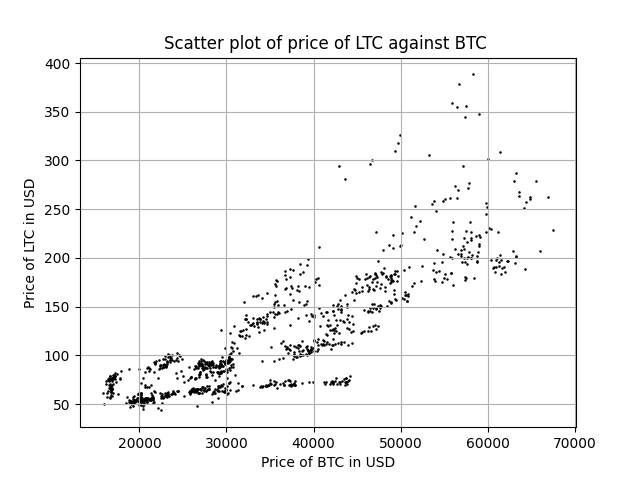
\includegraphics[width = \columnwidth]{Projects/TimeSeriesAnalysis/WrittenReport/plots/btcLtc.png}
    \caption{Scatter Plot of BTC and LTC prices, Jan '21 to Dec '23.\\
    \begin{centering}
        $\rho_p = 0.842$\\
        $\rho_s = 0.844$\\
    \end{centering}
    }
    \label{btc-ltc}
\end{figure}

\begin{figure}
    \centering
    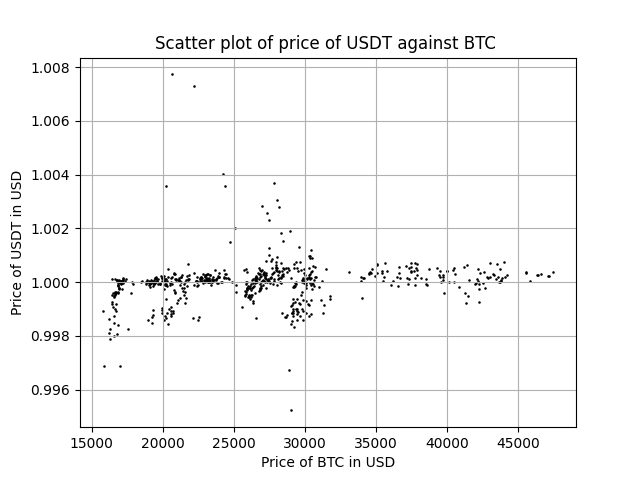
\includegraphics[width = \columnwidth]{Projects/TimeSeriesAnalysis/WrittenReport/plots/btcUsdt.png}
    \caption{Scatter Plot of BTC and USDT prices, Jan '21 to Dec '23.\\
    \begin{centering}
        $\rho_p = 0.165$\\
        $\rho_s = 0.329$\\
    \end{centering}
    }
    \label{btc-usdt}
\end{figure}

The cross-correlation plot is shown in Fig. \ref{crosscorr}.
\begin{figure}
    \centering
    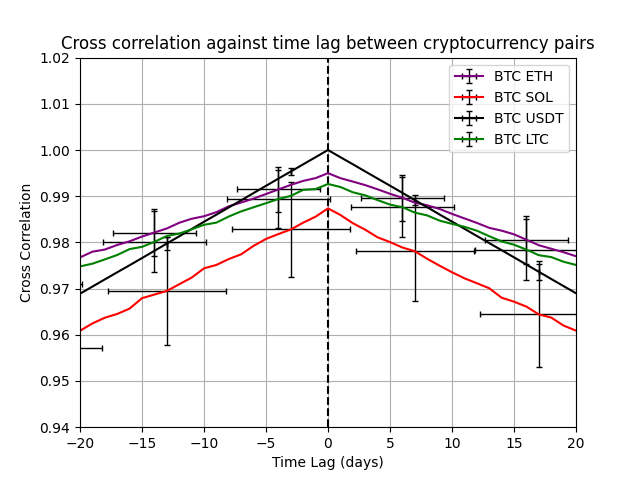
\includegraphics[width = \columnwidth]{Projects/TimeSeriesAnalysis/WrittenReport/plots/cross_correlation_main.png}
    \caption{Cross correlation across cryptocurrency pairs (BTC-X) of their prices from Jan '21 to Dec '23.}
    \label{crosscorr}
\end{figure}
The final values of the time-lag are:\\
\begin{table}[H]
    \centering
        \begin{tabular}{|c|c|c|}
             \hline
             Pair & Time Lag, $\tau$ (days) & Std. Dev. (days) \\
             \hline
             \hline
             BTC-ETH & $0\pm0.0684$ & $3.20$ \\
             \hline
             BTC-SOL & $0\pm0.124$ & $4.92$ \\
             \hline
             BTC-LTC & $0\pm0.0874$ & $4.21$ \\
             \hline
             BTC-USDT & $0\pm0.000$ & $0.00$ \\
             \hline
       \end{tabular}
     \label{tablevalues}
     \caption{Numerical values of the time lag of cryptocurrency pairs.}
\end{table}

\subsection{Correlation and time-lag of BTC and other things}\label{extras}
The relationship of BTC and search popularity was investigated. The search popularity is a relative measurement, where 100 is the peak popularity of the search term. The scatter plot and time-lag plot is shown in Fig. \ref{btc-search}. Fig. \ref{btc-gold} is for BTC-XAU and Fig. \ref{btc-eur} is for BTC-SPX. Finally, \ref{btc-snp} is BTC-SPX.
\begin{figure}
    \centering
    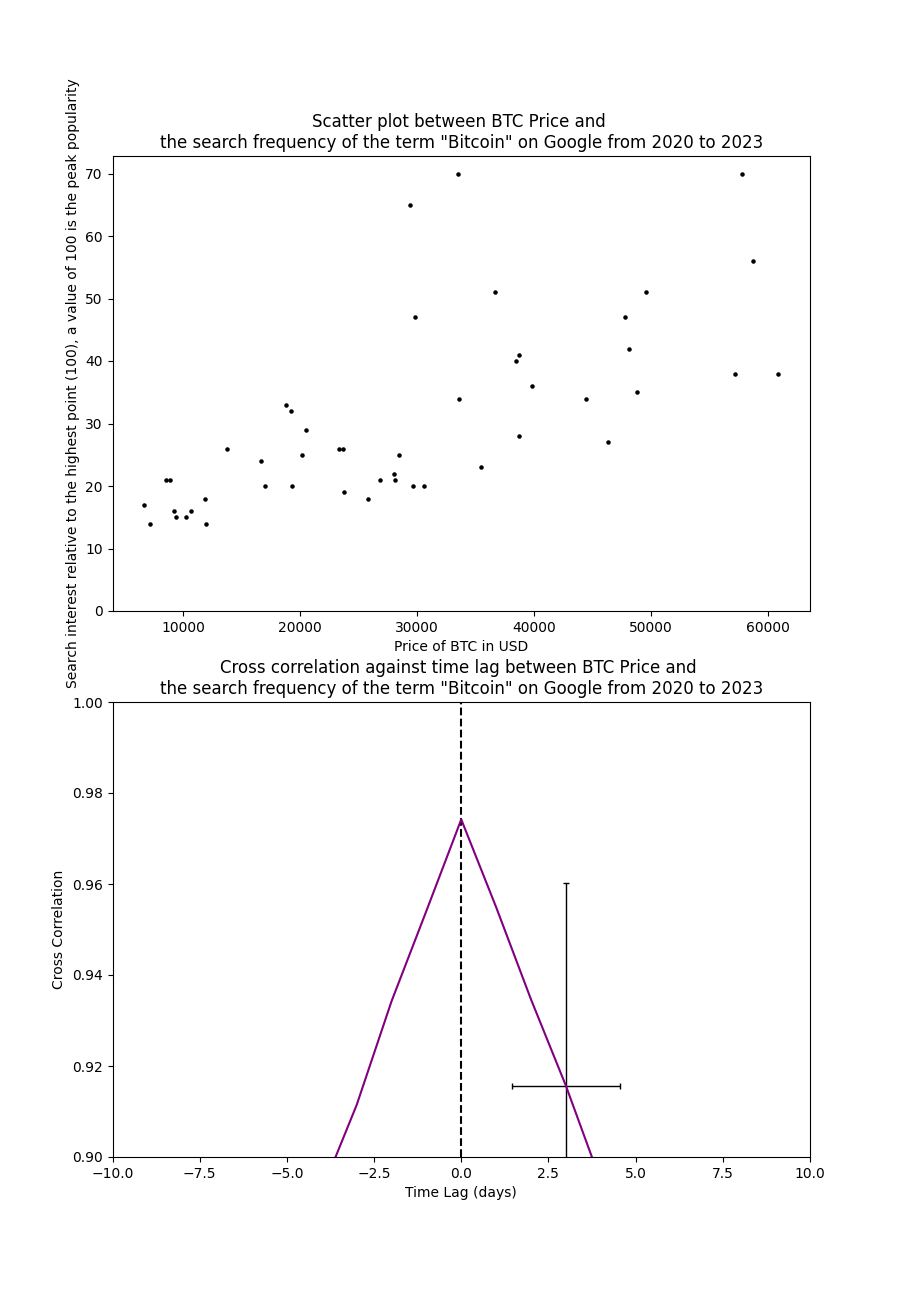
\includegraphics[width =\columnwidth]{Projects/TimeSeriesAnalysis/WrittenReport/plots/btcPricebtcSearch.png}
    \caption{Scatter and cross-correlation plots for BTC and BTC popularity by means of Google search frequencies.\\
        \begin{centering}
        $\rho_p = 0.682$\\
        $\rho_s = 0.776$\\
        $\tau = 0 \pm 0.162$ days\\
        $\sigma_\tau = 1.60$ days\\
    \end{centering}
    }
    \label{btc-search}
\end{figure}

\begin{figure}
    \centering
        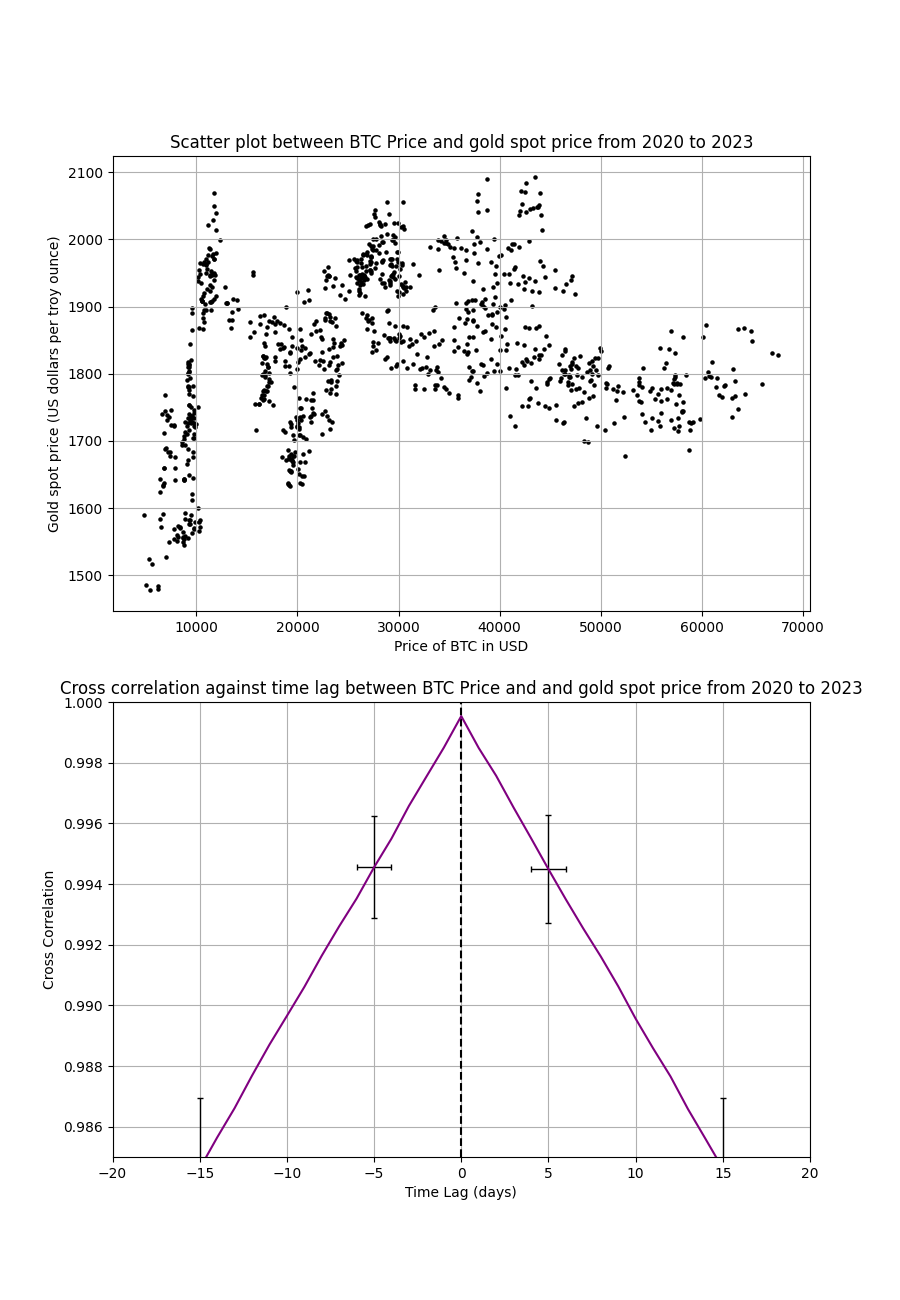
\includegraphics[width = \columnwidth]{Projects/TimeSeriesAnalysis/WrittenReport/plots/btcPriceGoldPrice.png}
        \caption{Scatter and cross-correlation plots for BTC and gold spot price.\\
        \begin{centering}
            $\rho_p = 0.213$\\
            $\rho_s = 0.196$\\
            $\tau = 0 \pm 0.0217$ days\\
            $\sigma = 1.59$ days\\
        \end{centering}
        }
        \label{btc-gold}
\end{figure}

\begin{figure}
    \centering
        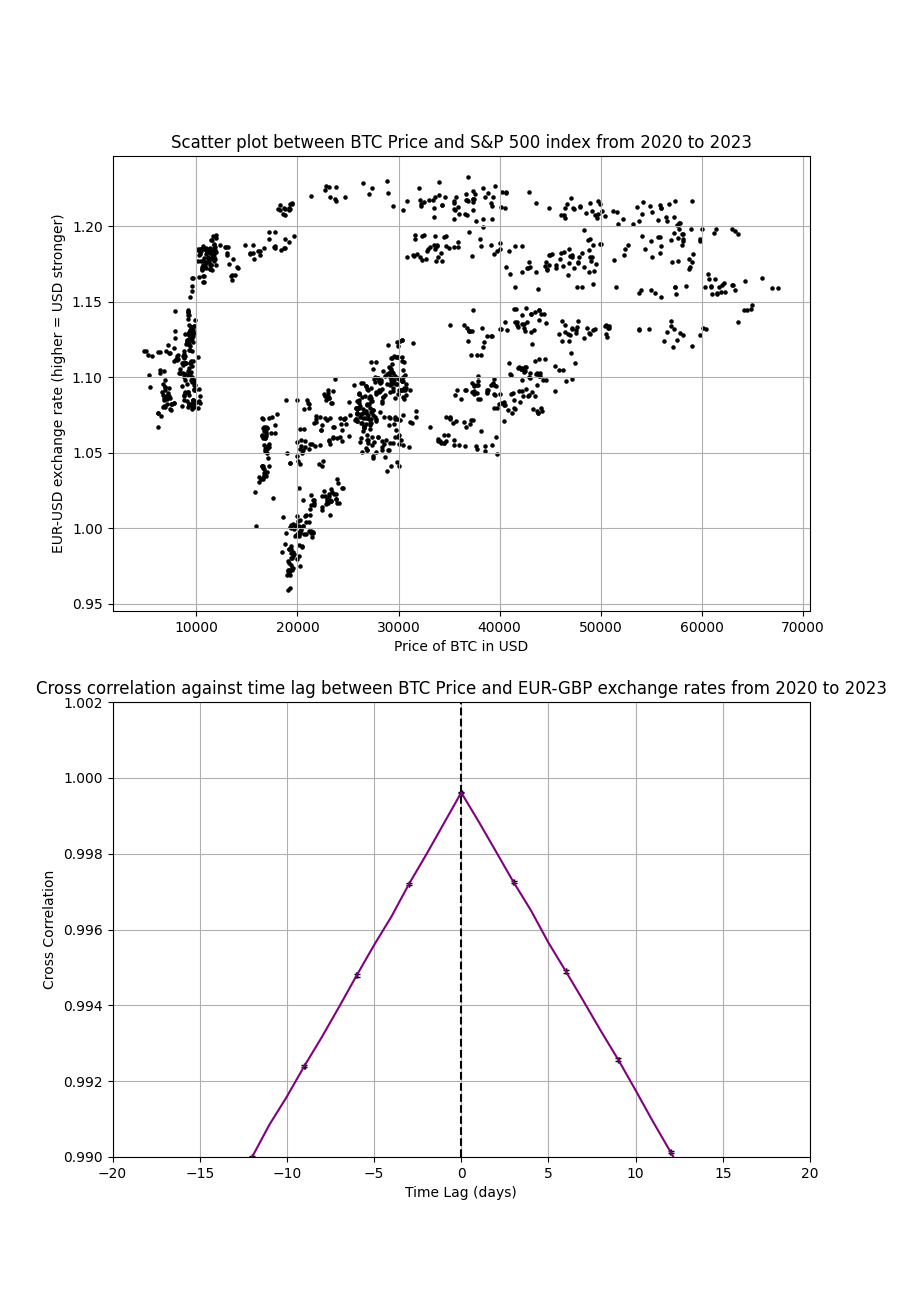
\includegraphics[width = \columnwidth]{Projects/TimeSeriesAnalysis/WrittenReport/plots/btcPriceEur.png}
        \caption{Scatter and Cross-correlation plots for BTC and EUR-USD exchange rate.\\
        \begin{centering}
            $\rho_p = 0.340$\\
            $\rho_s = 0.322$\\
            $\tau = 0 \pm 0.0194$ days\\
            $\sigma = 0.959$ days\\
        \end{centering}
        }
        \label{btc-eur}
\end{figure}

\begin{figure}
    \centering
    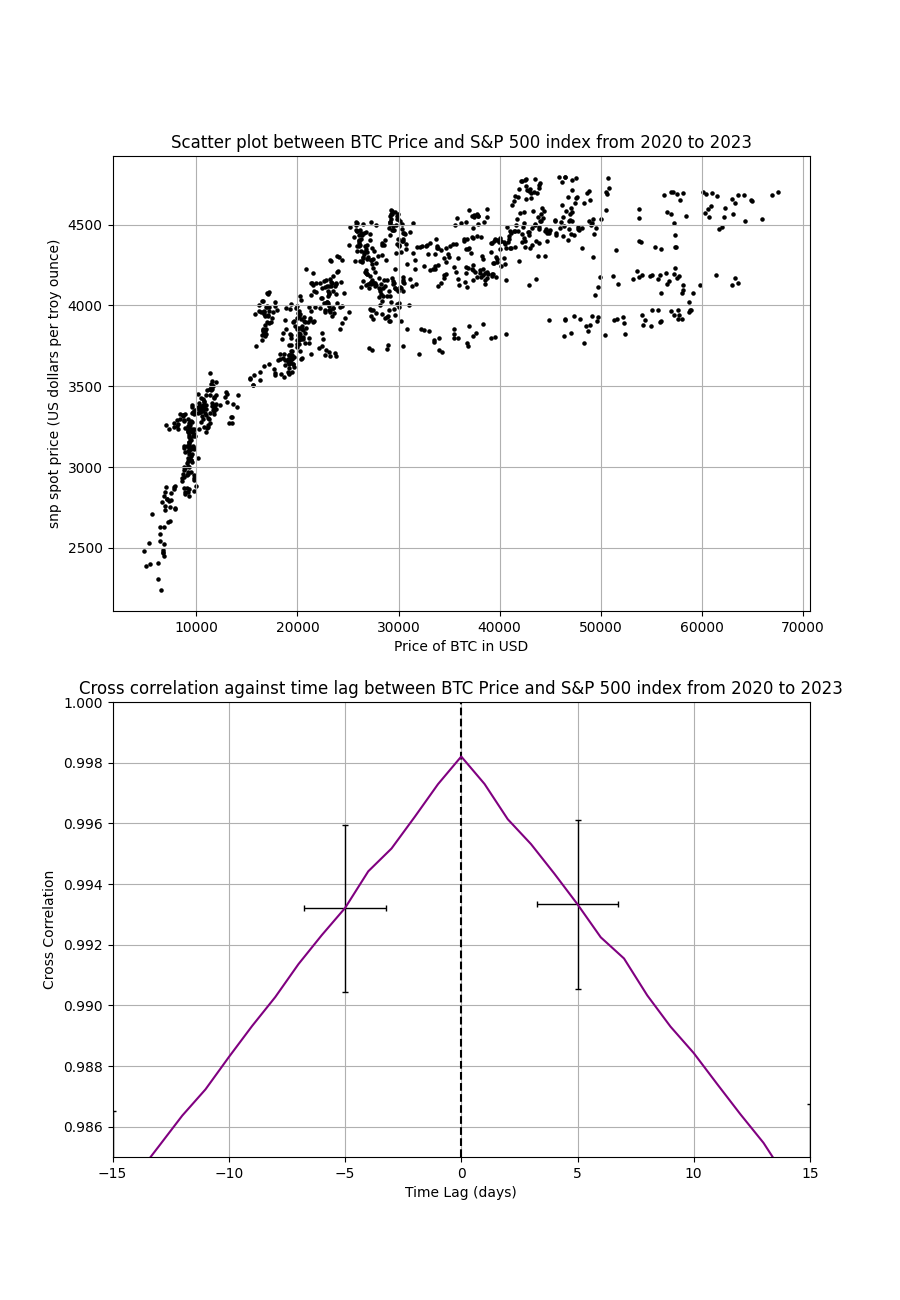
\includegraphics[width = \columnwidth]{Projects/TimeSeriesAnalysis/WrittenReport/plots/btcPriceSnp.png}
    \caption{Scatter and Cross-correlation plots for BTC and the S\&P500 index.\\
        \begin{centering}
        $\rho_p = 0.770$\\
        $\rho_s = 0.803$\\
        $\tau =  0 \pm 0.0394$ days\\
        $\sigma = 1.69$ days\\
    \end{centering}
    }
    \label{btc-snpg}
\end{figure}
\subsection{Summary of Results}
In the table below, I summarise the relationship between BTC-X pairs and the time-lags of the pairs.
\begin{table}[H]
    \centering
        \begin{tabular}{|c|c|c|}
            \hline
             Exchange pair & Relationship & Time Lag (days) \\
             \hline
             \hline
             BTC-ETH & Positive Monotonic & $0\pm0.0684$ \\
             \hline
             BTC-SOL & Positive Linear & $0\pm0.124$ \\
             \hline
             BTC-LTC & Positive Monotonic & $0\pm0.0874$ \\
             \hline
             BTC-USDT & None & $0\pm0.000$ \\
             \hline
             BTC-Search & Positive Monotonic & $0 \pm 0.162$ \\
             \hline
             BTC-XAU & None & $0 \pm 0.0217$ \\
             \hline
             BTC-EURUSD & None & $0 \pm 0.0194$ \\
             \hline
             BTC-SPX & Positive Monotonic & $0 \pm 0.0394$\\
             \hline
        \end{tabular}
    \caption{Summary of the relationships and time lag between BTC-X pairings.}
    \label{summaryvals}
\end{table}

\section{Analysis}
Most of the cryptocurrency pairings were positively monotonic ($\rho\sim1$) except for BTC-USDT. This is expected as the value of the USDt coin is pegged to the USD, whereas the value of the other coins in the pairings were linked to other factors. The relationships of the other coins are positive monotonic with very little time lag (based on the errors). On other factors, I conclude that there is only positive relationship between BTC prices with the search popularity and the S\&P500. 

From my findings, there is no significant lead-lag relationship (on the order of days), but there is an error on the time lag of $\pm\sim1.64$ hours. This is in line with the findings in \cite{Sifat2019}, although it was concluded that there was no lead-lag relationship between BTC and ETH, they also concluded that there was some merit for intra-day traders to exploit this small time lag difference. My hypothesis on BTC-USDT were also accurate as there was no relationship and no time-lag founded between the two.

The search popularity of BTC had a positive effect on the price of BTC, but there was no relationship founded on the EUR-USD exchange rate and BTC, as well as BTC-XAU, contrary to \cite{Georgoula2015}. Also, BTC was positively correlated to the S\&P500 index, an indicator of the global economy, which is also opposite from the findings in \cite{Georgoula2015}.

\section{Conclusion}
In this project, I investigate the prices of BTC against various coins and indexes, where the price data is the daily closing prices taken from January 2021 to December 2023 to investigate the effects on the COVID-19 pandemic. I conclude that BTC has a positive monotonic relationship and 0-day lag with most popular cryptocurrencies except for coins tied to "real" currencies such as USD. BTC was found to not have any relationship to the spot price of gold and the EUR-USD exchange rate, but a positive monotonic relationship and 0-day time lag with the S\&P500 index and the search frequency on Google. 

\section{Addendum}{\label{addendum}}
This section outlines the last 3 concepts studied in PHYS6017: integration, Runge-Kutta methods and Fourier transforms. A brief description of each is stated before some examples in and out of academia are given.
\\
\subsection{Integration}
A widely used mathematical concept, integration in a graphical representation is to find the area under the curve.
\\
\subsubsection{In Academia}
In Physics, path integrals are used heavily in classical and quantum mechanics. Maxwell's equations (in integral form) are so powerful in describing the world of electromagnetism. The Gauss integral is used in \cite{Rogen2003} to classify protein structure 
\\
\subsubsection{Outside of Academia}
Integrals (special integrals, to be exact) are incorporated into the world of economics \cite{Sherdor2023} in solving problems related to economic stability and market analysis. Fractional calculus (non-integer order differentiation, integration, summations) \cite{Ross1977} are used heavily in economics and have been used in the "Memory revolution" - an economic theory that takes into account the memory in economic processes \cite{Tarasov2019}. 
\\
\subsection{Runge-Kutta Method} %COMPLETE
The Runge-Kutta (RK) method is an iterative numerical method used to solve (commonly) non-linear differential equations, usually ill-posed. 
\\
\subsubsection{In Academia} %COMPLETE
The Runge-Kutta segmentation network (RKSeg) developed in \cite{Zhu2023} used the Runge-Kutta method to segment organ image datasets which outperformed other segmentation networks. In \cite{Jday2023}, an adaptive RK method was developed to solve the Cauchy problem\footnote{The solution of a partial differential equation defined in $\mathbb{R}^{n+1}$, where $n$ is the number of dimensions} of a modified Helmholtz equation. This ill-posed problem is hard to solve using "traditional" numerical methods, so using RK method is the way to go. The two-dimensional Riez-space fractional complex Ginzburg-Landau\footnote{A mathematical physical theory used to describe superconductivity, superfluidity and Bose-Einstein condensation. See \url{https://en.wikipedia.org/wiki/Ginzburg\%E2\%80\%93Landau_theory} and \cite{Aranson2002}} equations \cite{Wang2018} were solved using the exponential RK method \cite{Hochbruck2005}\cite{Hochbruck2010}.
\\
\subsubsection{Outside of Academia} %COMPLETE
RK method is practical for real-world scenarios as it is good at solving non-linear differential equations (which what most of the real world is), and it can be used in data science with data interpolation, as shown in \cite{Karim2018}. Traffic flow equations can be solved with RK methods, which have been summarised in \cite{Naja2022}. For example, the macroscopic model of traffic (where traffic flow is taken to act like a fluid), which is expressed as a differential equation \cite{Lighthill1955}\cite{Nagatani2002}: 
\begin{equation}
    \frac{\partial{\rho}}{\partial{t}} + \frac{\partial(f)}{\partial{x}}
\end{equation}
In \cite{Asri2021}, the Rubella vaccine's effect was analysed using RK-4 and RK-5 method in solving the SEIRS (Susceptible, Exposed, Infected, Recovered, Suspected) Model, showing that RK-5 method was better than RK-5 in predicting the rate of the Rubella disease spread. 
\\
\subsection{Fourier Transform} %COMPLETE
Fourier transforms, not to be confused with a Fourier series (where a function is written in terms of sums of exponential or sine and cosine functions) allows the time domain of a signal, periodic or otherwise to be expressed in the frequency domain (along with another phase component), and vice versa. Fast Fourier transforms (FFT) are used in most situations, i.e. in computing due to the number of operations needed. FFTs took $N\log{N}$ operations, compared to $N^2$ operations that the old FT algorithms took \cite{Cooley1969}.
\\
\subsubsection{In Academia} %COMPLETE
FFTs, along with convolution theory can be used by home security devices in smart homes to analyse the audio recorded, shown in \cite{Vadeiadis2020}, which shows the potential of intruder detection by smart home systems. In \cite{Hu1992}, 3-D random rough surfaces are simulated by using a 2-D digital filter, by introducing a method using spectrum analysis to calculate filter coefficients while employing the FFT for efficient filter implementation, similarly, FTs are used in describing the overall shape and ruggedness of particles in \cite{Wettimuny2004}. \cite{Orzechowski2019} explored the FT as an extension of the Black-Scholes-Merton Model in the context of pricing options.
\\
\subsubsection{Outside of Academia} %COMPLETE
In audio engineering, when taking acoustic measurements of audio devices, an FFT is applied onto the signal captured by a measurement microphone, which shows measurement graphs that tell the sonic characteristics of the drivers\footnote{Example: \url{https://crinacle.com/graphs/headphones/sennheiser-hd800s/}}. FFT is also used in music production with the same idea, by allowing the mixing engineer to visualise a waveform in the form of frequency spectrum and amplitude. In the same realm of audio engineering, FFTs are used to calculate the HRTF (Head Related Transfer Functions)\footnote{HRTFs characterise how an individual perceives sound. Due to the different physical properties of each individual, having a personalised HRTF is beneficial in immersive audio \cite{Oehler2023}.}, for example, to allow real-time spatial representation of moving sound sources in \cite{Tsakostas2007}.  In \cite{Nogata2012}, Fourier analysis is used to detect and visualise heart sounds using an FFT image and wavelet image that allows physicians to detect any abnormal heart sounds, showing that this could be used to develop an automatic detection system. 


\newpage
\section{Bibliography}
\bibliographystyle{apalike}
\bibliography{ref}
\section{Abbreviations}
The abbreviations below are used in this manuscript:
\begin{itemize}
    \item BTC - Bitcoin
    \item ETH - Ethereum
    \item SOL - Solana
    \item USDT - Theter USDt
    \item USD - United States Dollar
    \item SPX - S\&P 500 Index symbol
    \item XAU - Gold spot price symbol, in USD per troy ounce
    \item FT - Fourier Transform
    \item DFT - Discrete Fourier Transform
    \item FFT - Fast Fourier Transform
\end{itemize}
\\
The abbreviations below are used in the Addendum (Section \ref{addendum}):
\begin{itemize}
    \item RK - Runge Kutta
    \item FT - Fourier Transform
    \item FFT - Fast Fourier Transform
    \item HRTF - Head Related Transfer Function
\end{itemize}
\end{document}